\documentclass[12pt]{article}
\usepackage[utf8]{inputenc}
\usepackage[T1]{fontenc}
\usepackage{graphicx}
\usepackage{amsmath}
\usepackage{hyperref}
\usepackage{geometry}

\usepackage{graphicx} % Required for inserting images
\usepackage{mathtools,amsthm,amssymb,icomma,upgreek,xfrac}

\usepackage[all]{nowidow}
\usepackage[table]{xcolor}
\usepackage{amsmath}
\usepackage[utf8]{inputenc}
\usepackage{polski}
 


\geometry{
    top=1.8cm,
    bottom=2.5cm,
    left=2.5cm,
    right=2.5cm
}
\title{Komputerowa Analiza Szeregów Czasowych \\ 
\textbf{Analiza danych rzeczywistych przy pomocy modelu ARMA} }
\author{Prowadzący: mgr inż. Justyna Witulska \\  Autorzy: Zuzanna Nasiłowska i Maria Nowacka}
\date{31 stycznia 2025 r.}

\begin{document}
\maketitle

\section{Wstęp}
\subsection{Cel pracy}
Celem niniejszej pracy jest przeprowadzenie analizy rzeczywistych danych dotyczących globalnych temperatur w oparciu o model ARMA. Model ten łączy w sobie dwa podejścia: autoregresję (AR), która uwzględnia zależności pomiędzy obserwacjami w serii czasowej, oraz średnią ruchomą (MA), która uwzględnia wpływ losowych zakłóceń na zmienne w czasie. Dzięki temu możliwe jest uchwycenie zarówno systematycznych wzorców, jak i nieregularnych fluktuacji występujących w danych.Wykorzystanie tej koncepcji ma na celu zrozumienie dynamiki zmian temperatur na przestrzeni ostatnich 170 lat, w tym identyfikację długoterminowych trendów oraz sezonowych wahań. Analiza tego typu ma istotne znaczenie zarówno w kontekście badania zmian klimatycznych, jak i prognozowania przyszłych wartości temperatur, co może być pomocne w 
planowaniu działań związanych z adaptacją do globalnych zmian klimatu.
Praca ta ma także na celu odpowiedź na kilka istotnych pytań badawczych: 
\begin{itemize}
    \item Czy dane historyczne dotyczące temperatur są stacjonarne, a jeśli nie, to jakie transformacje są konieczne, aby model ARMA mógł zostać zastosowany? 
    \item  Jakie czynniki wpływają na zmienność temperatur w skali globalnej i czy można wyodrębnić pewne charakterystyczne wzorce?
\end{itemize}
Ostatecznie, celem jest także wykorzystanie modelu ARMA do stworzenia prognozy temperatur na przyszłość, co może być szczególnie istotne w kontekście globalnego ocieplenia i jego skutków. Ważnym aspektem realizacji celu pracy będzie także analiza jakości i struktury danych, a także dokładne przedstawienie wyników w formie tabel, wykresów i opisów.
\subsection{Dane}
Dane, które zostaną poddane analizie, pochodzą z publicznego i dostępnego zbioru danych opublikowanych na stronie Kaggle: Global Temperature Records. Zbiór obejmuje około 170 lat pomiarów temperatury. Dane te zawierają miesięczne i roczne odczyty średnich temperatur globalnych, obejmujące zarówno temperatury powierzchni lądowej, jak i oceanicznej. W niniejszym raporcie skupimy się konkretnie na mieście \textbf{Aleksandria} położonym w Egipcie. Dane te zostały zebrane przez różne instytucje naukowe, co podkreśla ich wiarygodność i przydatność w analizach naukowych. Dokładna długość próby wynosi: \textbf{170}.
\\
\\ Dane są zorganizowane w formie tabelarycznej, gdzie każdemu rekordowi przypisane są następujące aspekty:
\begin{itemize}
    \item Data: Określa rok i miesiąc pomiaru.
    \item Średnia temperatura: Podana w stopniach Celsjusza, reprezentująca średnią globalną temperaturę dla danego okresu.
    \item Anomalia temperatury: Różnica między zmierzoną temperaturą a wartością referencyjną, co pozwala na identyfikację odchyleń od normy.
\end{itemize}
Wspomniane powyżej dane znajdują się pod następującym adresem:
\\ \href{https://www.kaggle.com/datasets/maso0dahmed/global-temperature-records-1850-2022}{Global Temperature Records 1850-2022}.

\subsection{Wizualizacja danych}
Pierwszym krokiem w analizie będzie wizualizacja danych, która pozwoli na wstępne zrozumienie ich struktury. W tej sekcji przedstawimy graficzne reprezentacje średnich temperatur w Aleksandrii, co umożliwi lepsze zrozumienie ich zmienności w czasie. Wykorzystamy do tego dwa podejścia:
\begin{itemize}
    \item \textbf{Mapa cieplna średnich miesięcznych temperatur} -> ta wizualizacja pozwoli na szybkie zidentyfikowanie ewentualnych anomalii w poszczególnych latach.
    \item \textbf{Wykres surowych danych} -> przedstawienie surowych danych w formie wykresu liniowego umożliwi obserwację trendów i fluktuacji temperatur w dłuższym okresie.
\end{itemize}

\begin{figure}[!htbp]
\hspace*{0 cm}
	\centering
	\includegraphics[scale=0.50]{heatmapka.png}
	\caption{Mapa cieplna średnich temperatur w Aleksandrii}
\end{figure}

\begin{figure}[!htbp]
\hspace*{0 cm}
	\centering
	\includegraphics[scale=0.50]{surowe.png}
	\caption{Wykres surowych danych}
\end{figure}

\section{Przygotowanie danych do analizy}
\subsection{Badanie jakości danych}
% (opcjonalnie) wyodrębnienie z danych obserwacji do zbioru testowego,
\subsection{Dekompozycja szeregu czasowego}

\begin{figure}[!htbp]
    \centering
    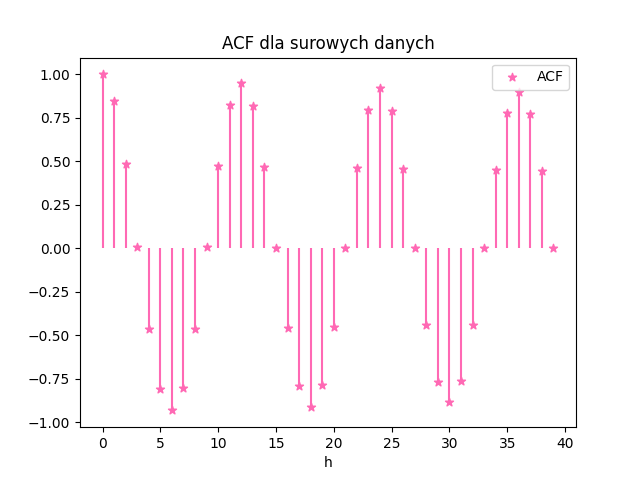
\includegraphics[scale=0.70]{surowe_acf.png}
    \caption{Wykres autokorelacji dla surowych danych}
    \label{fig:enter-label}
\end{figure}

% Na wykresie acf widać sezonowość
\begin{figure}[!htbp]
    \centering
    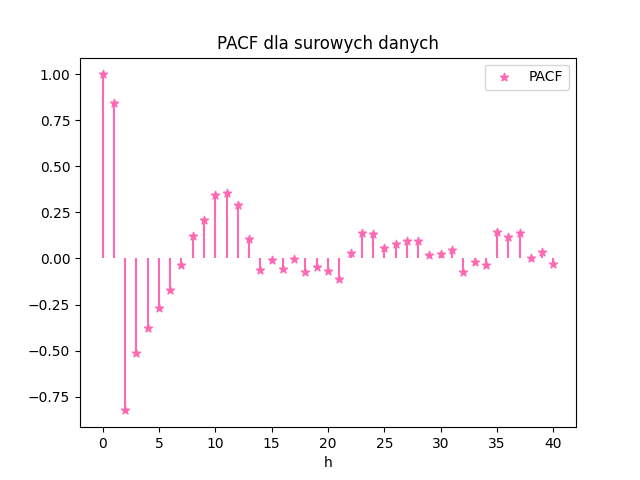
\includegraphics[scale=0.70]{surowe_pacf.png}
    \caption{Wykres PACF dla surowych danych}
    \label{fig:enter-label}
\end{figure}
% Na wykresie pacf również widać sezonowość
\\
% – (opcjonalnie) test ADF weryfikujący hipotezę o niestacjonarności dla surowych danych (Augmented Dickey-Fuller Test), \\

\begin{figure}[!htbp]
    \centering
    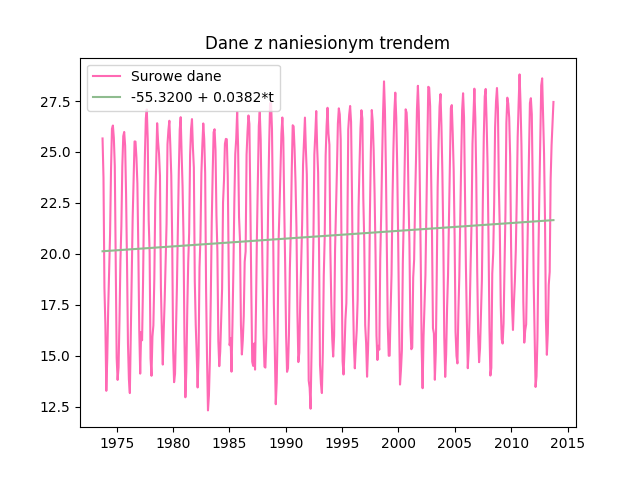
\includegraphics[scale=0.70]{daneItrend.png}
    \caption{Dane i widoczny trend}
    \label{fig:enter-label}
\end{figure}
Trend obliczony regresją liniową: -55.3200 + 0.0382*t \\
Dane bez trendu
\begin{figure}[!htbp]
    \centering
    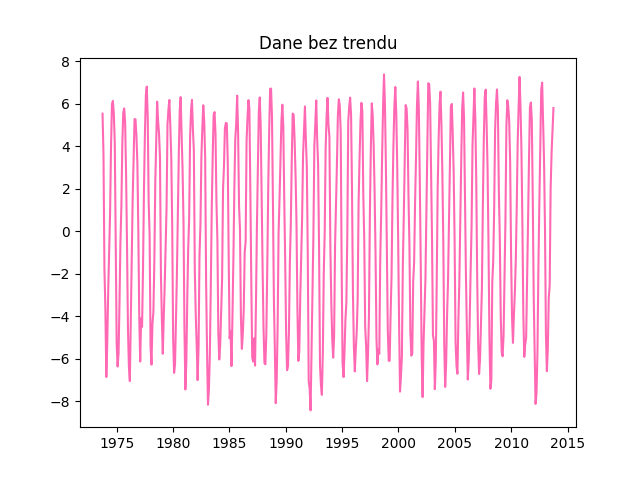
\includegraphics[scale=0.70]{dane_bez_trendu.png}
    \caption{Po usunięciu trendu}
    \label{fig:enter-label}
\end{figure}
Sezonowość: 6.3869*sin(6.2693t + 6.1977) \\
A * sin($\omega$t + c) \\
Okresowość: T = 12.001580899215833 [miesięcy], czyli w przybliżeniu rok.
– wykres ACF oraz PACF dla uzyskanego szeregu, 
\begin{figure}[!htbp]
    \centering
    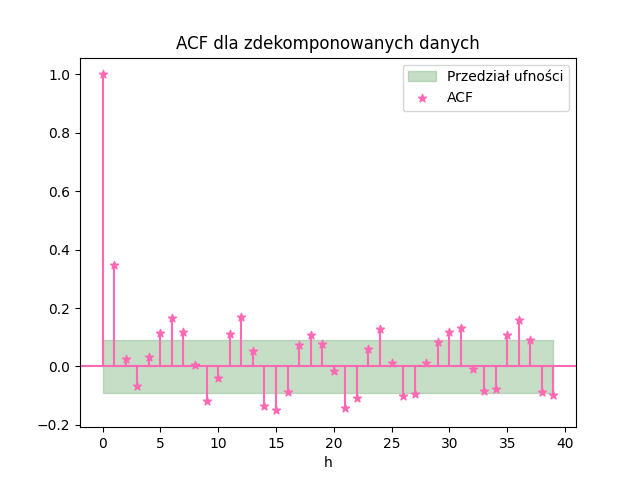
\includegraphics[scale=0.70]{decomposed_acf.png}
    \caption{Wykres autokorelacji dla danych poddanych dekompozycji}
    \label{fig:enter-label}
\end{figure}

\begin{figure}[!htbp]
    \centering
    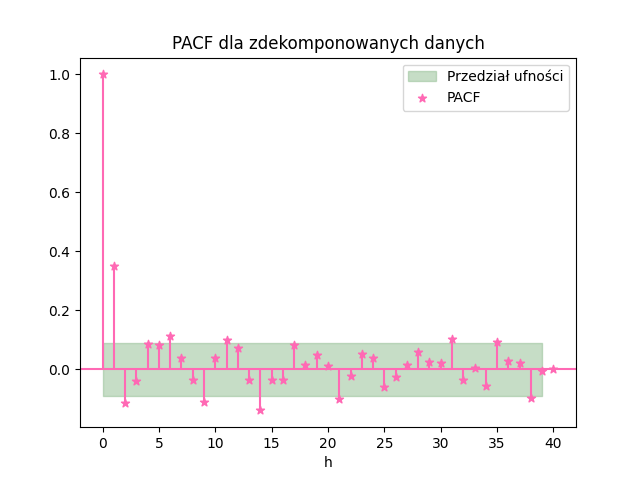
\includegraphics[scale=0.70]{decomposed_pacf.png}
    \caption{Wykres PACF dla danych poddanych dekompozycji}
    \label{fig:enter-label}
\end{figure}
\\
% – (opcjonalnie) test ADF weryfikujący hipotezę o niestacjonarności dla uzyskanego szeregu (Augmented Dickey-Fuller Test).

\section{Modelowanie danych przy pomocy ARMA}
\subsection{Dobranie rzędu modelu}
% tutaj mamy 2 wersje, zależy jak wyznaczamy to mamy ARMA(3,2) albo ARMA(4,2)
\subsection{Estymacja parametrów modelu}
dla ARMA(4,2) mamy \\
$\phi_1 = 1.381848025075898$, 
$\phi_2 = -1.309824869304384,$  
$\phi_3 = 0.3435885988141824,$ 
$\phi_4 = 0.02076713721749783,$ \\
$\Theta_1 = -1.030694181786215,$ 
$\Theta_2 =  0.9218716219643841)$ \\
% Dla ARMA(3,2) mamy:
% (1.3294901979849114,
%  -1.330899499237904,
%  0.33176736127690115,
%  -1.003476675660714,
%  0.9996826747588954)
\begin{figure}[!htbp]
    \centering
    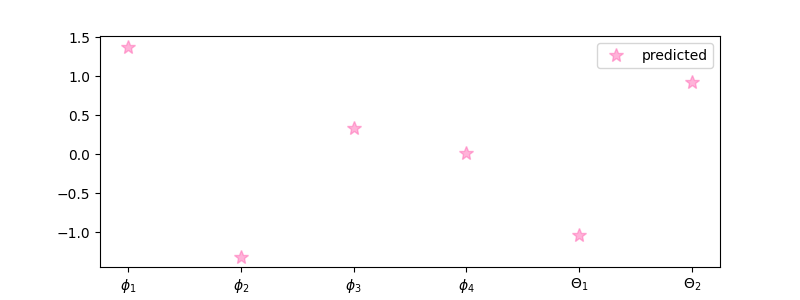
\includegraphics[scale=0.70]{params42.png}
    % \caption{}
    \label{fig:enter-label}
\end{figure}

\section{Ocena dopasowania modelu}
\subsection{Przedziały ufności}
\begin{figure}[!htbp]
    \centering
    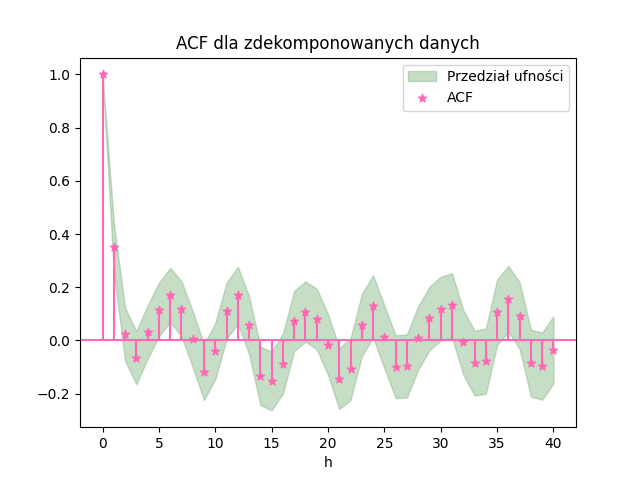
\includegraphics[scale=0.70]{przedzial_acf.png}
    % \caption{Wykres autokorelacji dla danych poddanych dekompozycji}
    \label{fig:enter-label}
\end{figure}

\begin{figure}[!htbp]
    \centering
    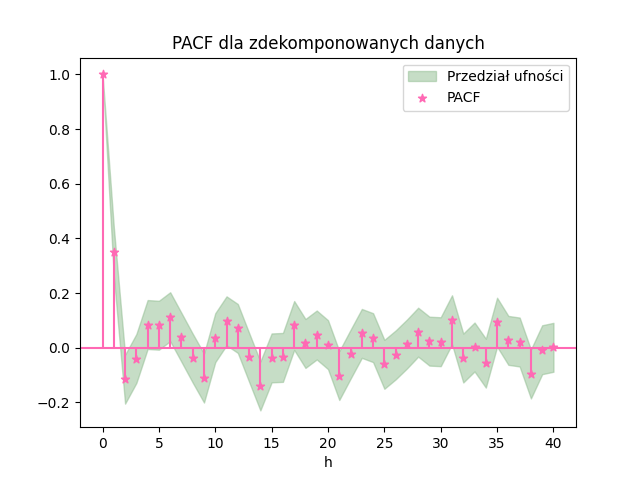
\includegraphics[scale=0.70]{przedział_pacf.png}
    % \caption{Wykres PACF dla danych poddanych dekompozycji}
    \label{fig:enter-label}
\end{figure}
\subsection{Porównanie linii kwantylowych z trajektorią}
% (opcjonalnie) prognoza dla przyszłych obserwacji i porównanie z rzeczywistymi danymi.


\section{Weryfikacja założeń dotyczących szumu}
\begin{figure}[!htbp]
    \centering
    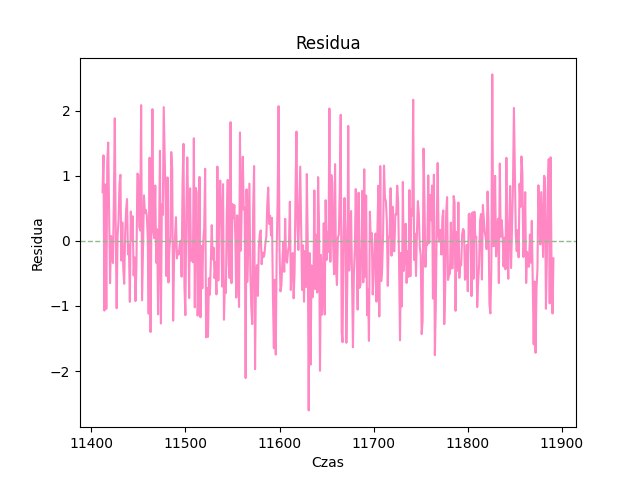
\includegraphics[scale=0.70]{residuals.png}
    % \caption{}
    \label{fig:enter-label}
\end{figure}
\subsection{Średnia}
Obliczona średnia to: 0.0007688935697969394 - jest bliska zeru. \\
Wykres (ten co wyżej) + ttest \\
t-statistic: 0.019071340621541755, p-value: 0.9847921354320044 \\
Brak podstaw do odrzucenia hipotezy zerowej. Średnia nie różni się istotnie od wartości oczekiwanej.

\subsection{Wariancja}
Wykres (ten co wyżej)  + Arch test \\
Lagrange Multiplier Test Statistic: 16.76695795645801 \\
LM Test p-value: 0.07968229620638863 \\
F-Test Statistic: 1.6980301496365462 \\
F-Test p-value: 0.07848236817609255 \\
Brak podstaw do odrzucenia hipotezy zerowej: Brak efektu ARCH.
% czyli jest git
\subsection{Niezależność}
Wykres ACF/PACF + / test Ljunga-Boxa \\
\begin{figure}[!htbp]
    \centering
    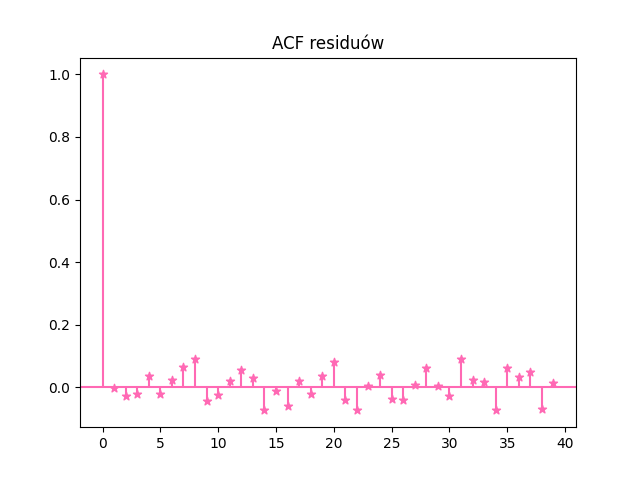
\includegraphics[scale=0.70]{resid_acf.png}
    % \caption{}
    \label{fig:enter-label}
\end{figure}
%     lb_stat  lb_pvalue \\
% 10\  9.30411  \  0.503506 \\
p-value > 0.05, czyli są niezależne.

\subsection{Normalność rozkładu}
Dystrybuanta, gęstość + test
\begin{figure}[!htbp]
    \centering
    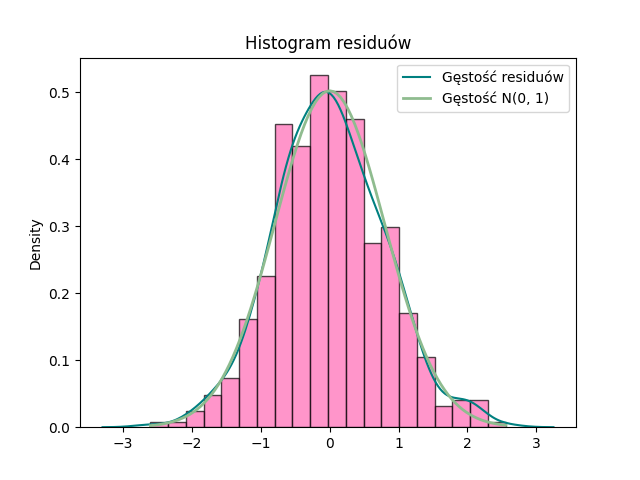
\includegraphics[scale=0.70]{norm.png}
    % \caption{}
    \label{fig:enter-label}
\end{figure}
% dla residuals
ShapiroResult(statistic=0.9966776967048645, pvalue=0.4291416108608246) \\
Więc przeszedł test na normalność
% dla X3
ShapiroResult(statistic=0.9958302974700928, pvalue=0.23462893068790436 \\
Też przechodzi test na normalność.

\section{Zakończenie}
\subsection{Podsumowanie}
\subsection{Wnioski}


\end{document}
